% Charlotte Geiger - Manuel Lippert - Leonard Schatt
% Physikalisches Praktikum

% Teilauswertung 2

\def\weite{4cm}

\section{Umkehrintegrator}
Bei der Betrachtung unserer Bilder am Oszilloskop wird deutlich, dass der Umkehrintegrator bei zunehmender Frequenz immer besser integriert und die dadurch entstehende Dreiecksspannung\\
\begin{center}
    \begin{tabular}{c c c}
        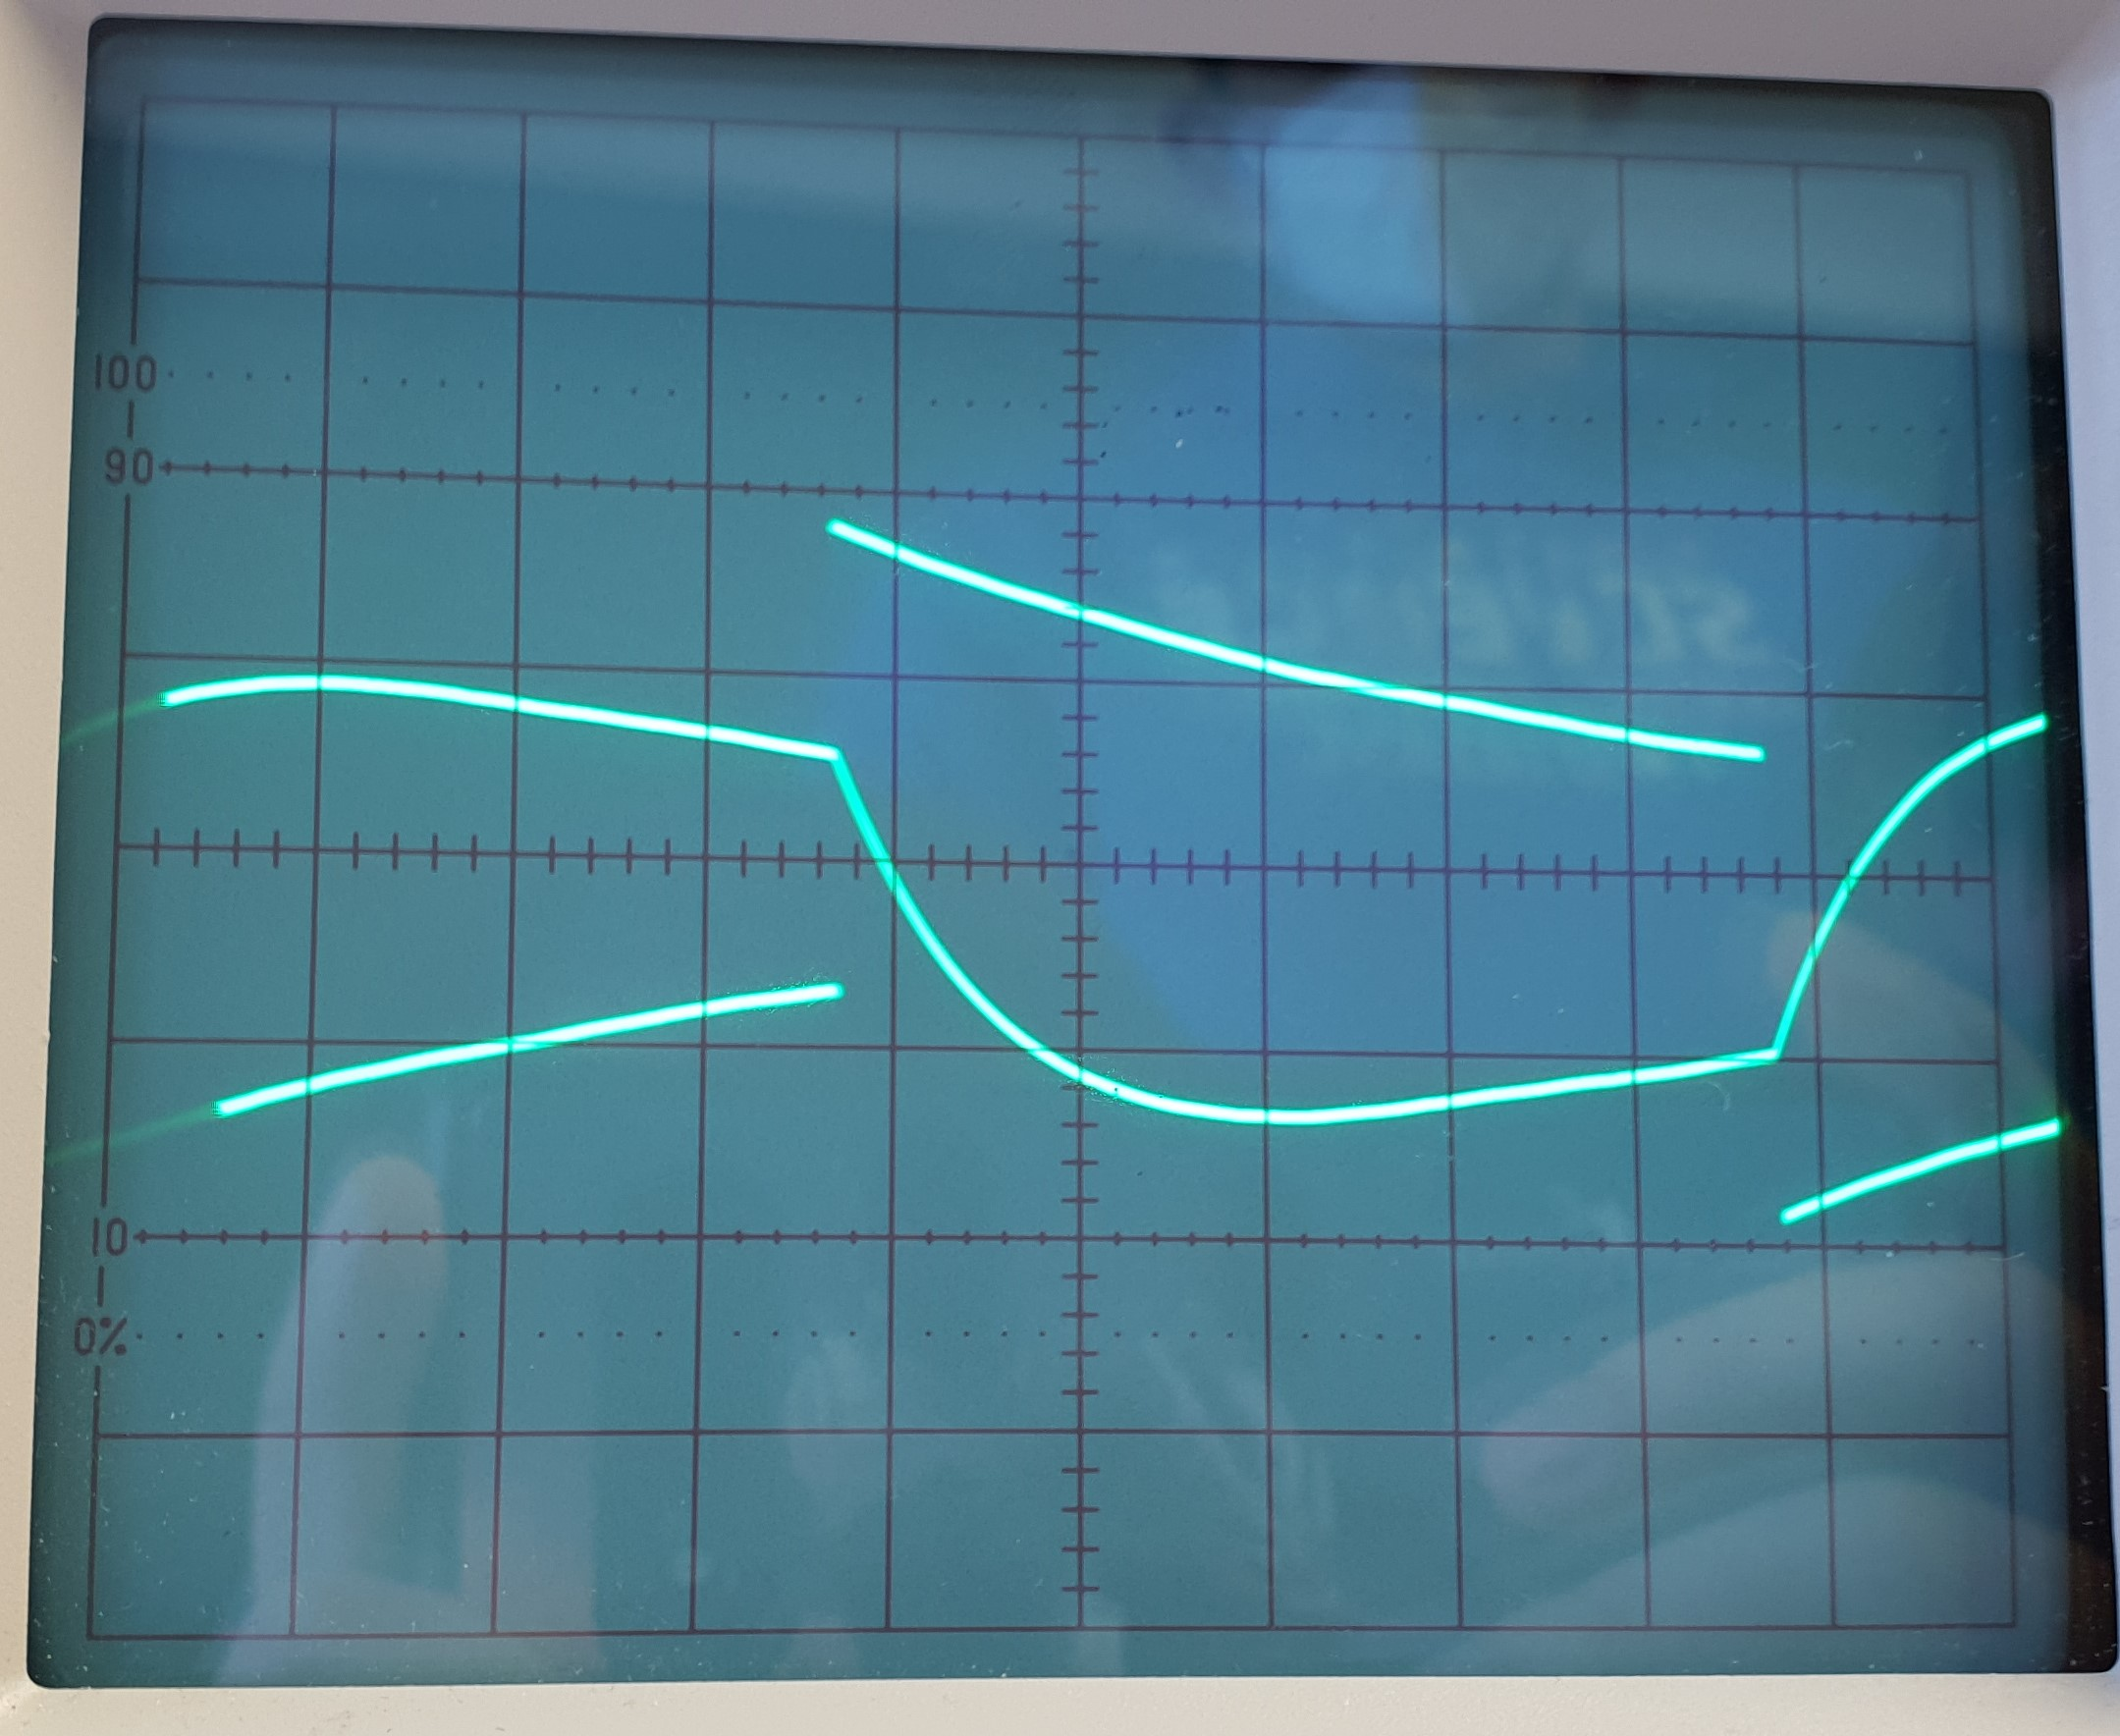
\includegraphics[width = \weite]{42-10Hz.jpg} & 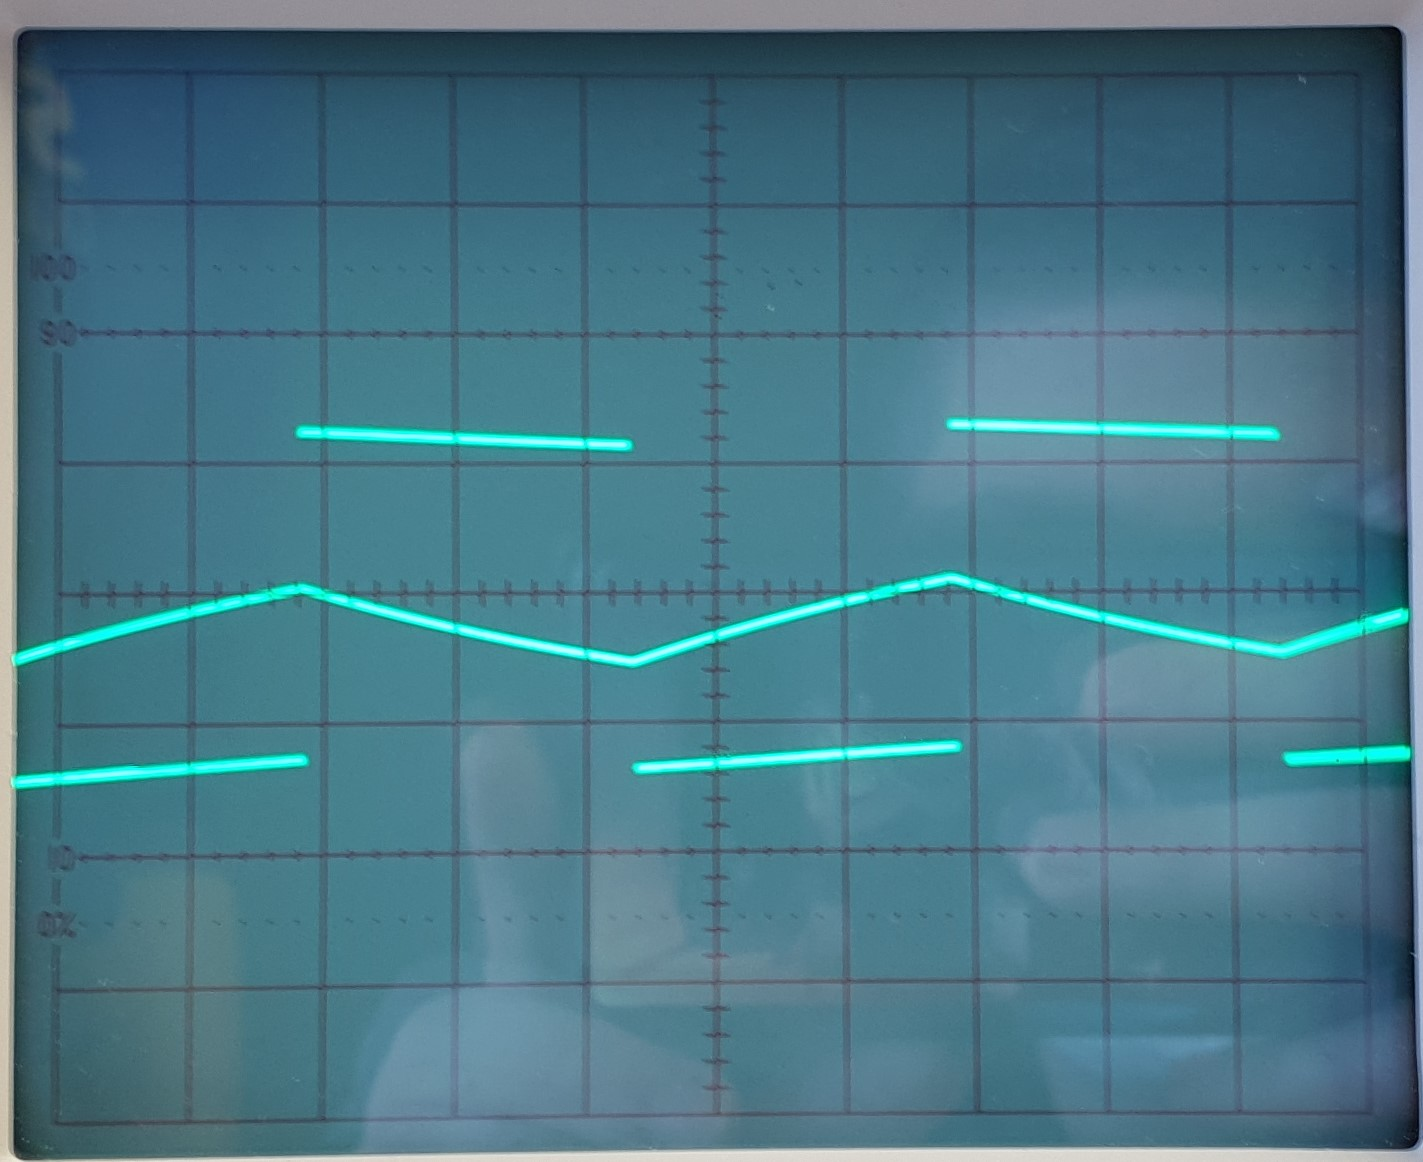
\includegraphics[width = \weite]{42-100Hz.jpg} & 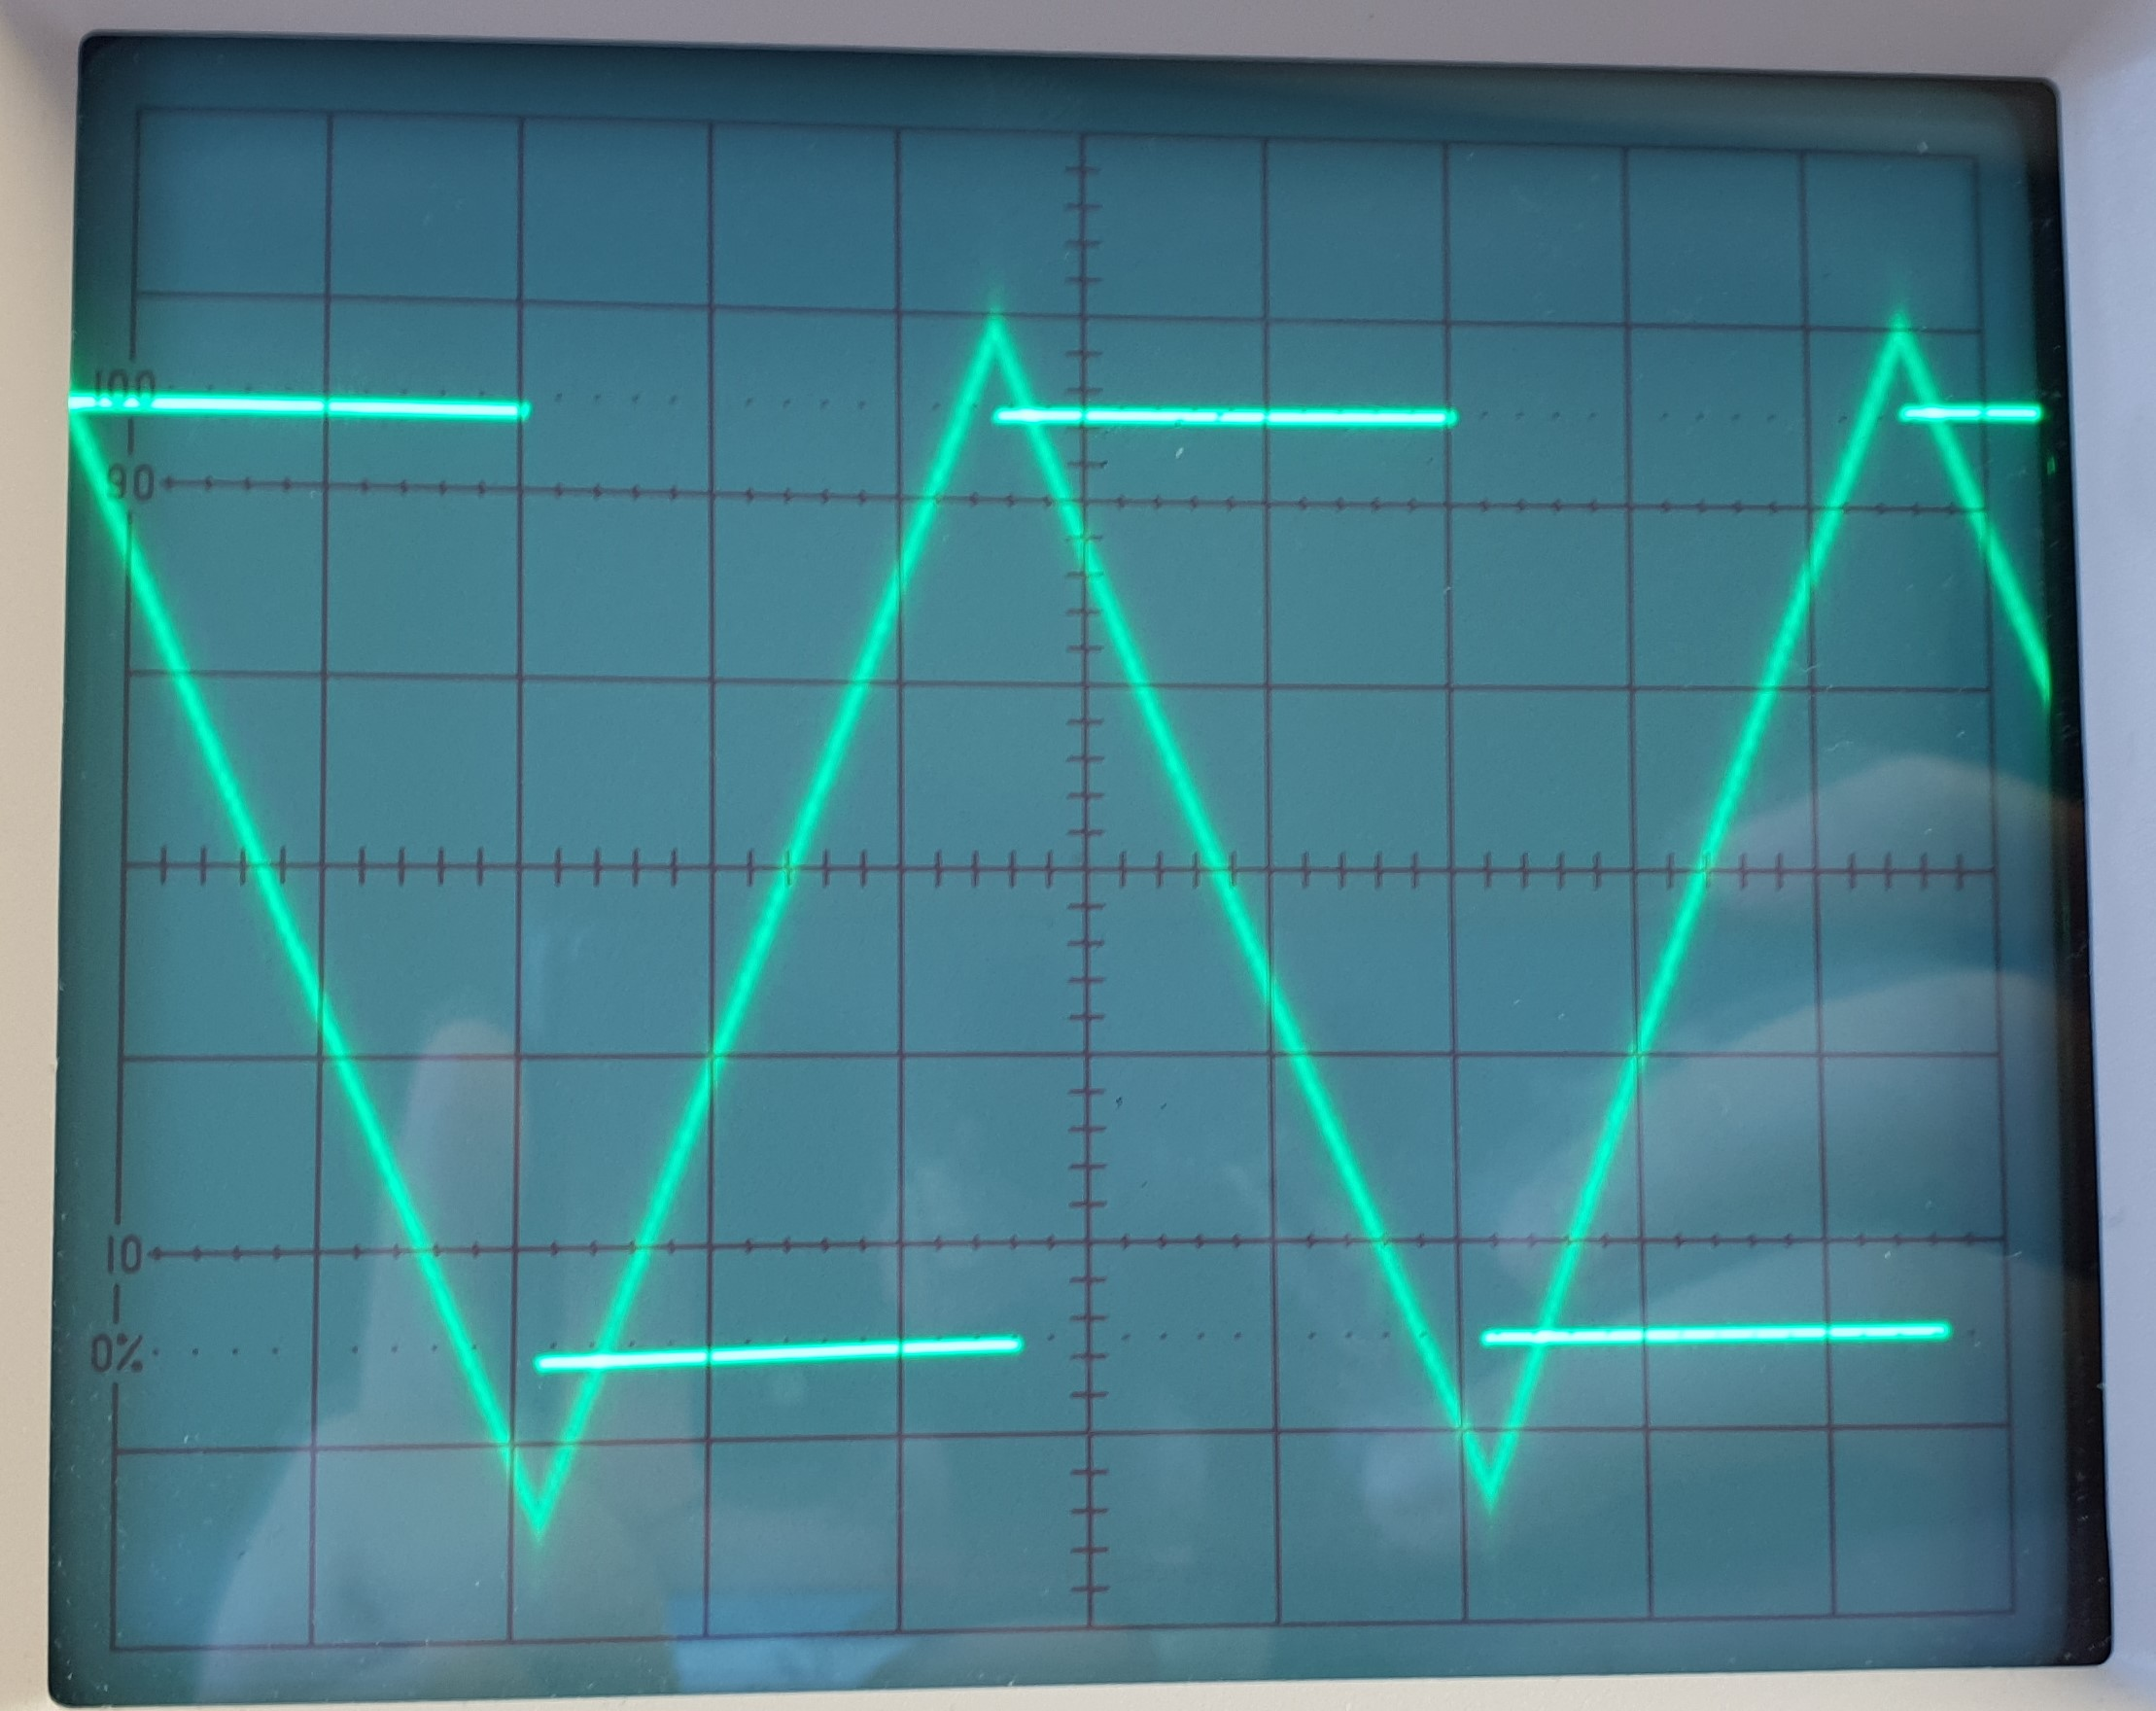
\includegraphics[width = \weite]{42-1000Hz.jpg}
    \end{tabular}
    \captionof{figure}{Test}
\end{center}